% TODO:
% 1. The MAA does not provide a Reference Service. 
% Please align the style of your references with the MAA Reference Style Guide. (See attached.)
% 2. Please enter the correct reference number here or compile the 
% TeX file before submitting. Here and elsewhere.
% 3. This Filler may be a bit too long. 
% You may need to remove one sentence. We can wait and see if you prefer.



%MSC Primary: XXXXX
\documentclass{article}
\usepackage{maa-monthly}

%\usepackage{tikz}

\raggedbottom
%\flushbottom
%\final

%\setcounter{annual}{XXXX}
%\setcounter{volume}{XXX}
%\setcounter{issue}{X}
%\setcounter{page}{XXX}

\allowdisplaybreaks

%\theoremstyle{theorem}
%\newtheorem{theorem}{Theorem}[section]

\theoremstyle{plain}
\newtheorem*{theorem}{Theorem}


\begin{document}
\begin{filler}
[white]
\noindent {\large \bf \textsf{The Expected Number of $n$-sided Dice Throws to Collect $k$ Points is a Geometric Series for $k\leq n$}}\\


\noindent Let's start with a visual proof of a formula for the sum of a  finite geometric series.
We consider a growing geometric series $(b_j)$ where $b_{j + 1} = r b_j$ with ratio $r > 1$.
We represent the ratio as $r = 1 + \alpha$, so $b_{j + 1} = b_j + \alpha b_j$.

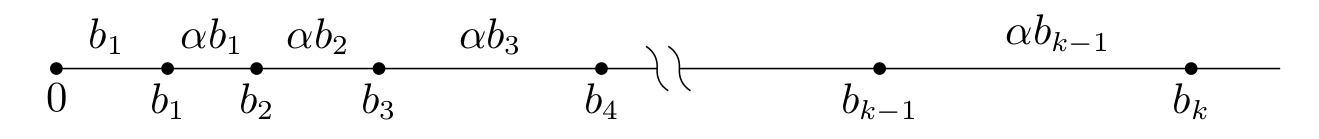
\includegraphics[width=11cm]{geometric_series.png}


% here is the tikz code for the picture
% \tikzset{ext/.pic={
% \path [fill=white] (-0.2,0)to[bend left](0,0.1)to[bend right](0.2,0.2)to(0.2,0)to[bend left](0,-0.1)to[bend right](-0.2,-0.2)--cycle;
% \draw (-0.2,0)to[bend left](0,0.1)to[bend right](0.2,0.2) (0.2,0)to[bend left](0,-0.1)to[bend right](-0.2,-0.2);
% }}

% \begin{tikzpicture}
% \foreach \Point/\PointLabel in {(0,0)/0, (1,0)/b_1, (1.8,0)/b_2, (2.9,0)/b_3, (4.9,0)/b_4, (7.4,0)/b_{k-1}, (10.2,0)/b_k}
% \draw[fill=black] \Point circle (0.05) node[below] {$\PointLabel$};
% \path [draw] (0,0)--pic [rotate=90]{ext}(11,0);

% \foreach \Point/\PointLabel in {(0.45,0)/b_1, (1.4,0)/\alpha b_1, (2.35,0)/\alpha b_2, (3.9,0)/\alpha b_3, (9.0,0)/\alpha b_{k-1}}
% \draw \Point node[above] {$\PointLabel$};
% \end{tikzpicture}
		

Adding all the segment lengths we see that
\[
b_{k} = b_1 + \alpha (b_1 + b_2 + b_3 + \ldots + b_{k-1}).
\]

This property of geometric series also has an economic intuition. 
Your final welfare $b_k$ equals your initial welfare $b_1$ plus all interest payments,
where $\alpha$ is the nominal rate of compound interest.


Now let's toss a $n$-sided dice until we collect $k$ points or more with $k\leq n$.
We denote the random number of tosses by $X_k$ and the expected number of tosses 
by $b_k = E(X_k)$. 

We collect one point or more with exactly one toss, $X_1 = 1$ and hence $b_1 = 1$. 

Now we need to collect $k$ points or more. Let's consider the first toss.
With probability $(n - k)/n$ zero more tosses will be required. 
And with probability $1/n$ we collect $1$, $2$, \ldots, or $k-1$ points.

The recurrence formula is
\[
b_k = 1 + \frac{n - k}{n} \cdot 0 + \frac{1}{n} (b_1 + b_2 + \ldots + b_{k-1}).
\]
This equation coupled with the initial conditions defines the geometric series with $b_1 = 1$ and ratio $r = 1 + \frac{1}{n}$.

Hence we obtain
\[
b_k = E(X_k) = \left( 1 + \frac{1}{n} \right)^{k-1}.
\]


This result appears in the disguised form $E(X_k) = \sum_{i=0}^{k-1} \binom{k-1}{i} / n^i$ in \cite{conroy2021collection}.
The particular case with $k=n$ is proven in \cite{trevino2020expected}.
Both these sources invoke the Christmas stockings theorem in their proofs.
The approach with recurrence equation is used in \cite{146114}, 
where the chase for the general $k$ hides the simple structure for $k\leq n$. 


\begin{thebibliography}{1}
\bibitem{conroy2021collection} Conroy, M (2021). A collection of dice problems. \url{www.madandmoonly.com/doctormatt/mathematics/dice1.pdf}.
\bibitem{trevino2020expected} Trevi{\~n}o, Enrique (2020). Expected Number of Dice Rolls for the Sum to Reach n. \textit{Amer. Math. Monthly}. 127(3):257-257.
\bibitem{146114} Usual Suspect (2019). Expected number of dice rolls require to make a sum greater than or equal to K? \url{https://stats.stackexchange.com/q/146114}.
\end{thebibliography}


\rightline{---Submitted by Boris Demeshev, HSE University}


\bigskip
\footnoterule
\footnotesize{doi.org/10.XXXX/amer.math.monthly.122.XX.XXX}

\footnotesize{MSC: Primary 00X00, Secondary 11Y11; 22Z22}

\end{filler}

\end{document}
